\documentclass[twoside]{report}

\usepackage{amsmath}
\usepackage{amssymb}
\usepackage{amsthm}

\usepackage{microtype}
\usepackage{booktabs}
\usepackage[thinlines]{easytable}
\usepackage[labelfont=bf]{caption}
\usepackage{centernot}
\usepackage[parfill]{parskip}

\usepackage{thmtools}
\usepackage[dvipsnames]{xcolor}
\definecolor{light-gray}{gray}{0.95}
\declaretheorem[shaded={bgcolor=light-gray}]{theorem}
\renewcommand{\qedsymbol}{$\blacksquare$}
\DeclareMathOperator{\mean}{mean}

\usepackage{multicol}
\usepackage{marginnote}

\usepackage{hyperref}
\usepackage{graphicx}
\usepackage{tikz}
\usepackage{pgfplots}

\pgfplotsset{width=2.25in}

\renewcommand*{\marginfont}{\sffamily\footnotesize}
\newcommand{\header}[2]{\begin{flushright} \textbf{#1} #2 \end{flushright}}

\usepackage[english]{babel}
\addto\captionsenglish{\renewcommand\chaptername{Note}}

\begin{document}

\title{\textsc{Introduction to Mathematical Proofs} \\
	\large at the University of Toronto}
\author{Hermish Mehta \\ University of California, Berkeley}
\date{\today}
\maketitle

\tableofcontents

\chapter{Numbers, Sets, and Functions}
\section{Quadratic Equations}
One of the simplest classes of equations we regularly solve are \emph{linear equations}, \marginnote{linear equations} equations of the form below, where the greatest power of our variable is one. As a matter of terminology, we denote the constants 

\begin{align}
	ax + b = 0 	
\end{align}

Solving this equation can be done by rearranging and then dividing both sides by $a$, yielding

\begin{align*}
	x = -\frac{b}{a}.
\end{align*}

Naturally, we may want to solve some more complicated \textit{quadratic equations}, \marginnote{quadratic equations} where the greatest power of our variable is two. Such equations take the general form

\begin{align}
	ax^2 + bx + c = 0.
\end{align}

To solve this equation, we need to isolate $x$ and in doing so, reduce the number of terms with the variable from two to one. This can be accomplished through a problem solving strategy called wishful thinking.

\begin{align*}
	a \left( x^2 + \frac{b}{a}x \right) + c
\end{align*}

Writing the left hand side of the equation like this, we can see by adding the right constant inside the parentheses, this can be reduced to a square. Returning to our original equation, this results in the following steps.

\begin{align*}
	0 &= ax^2 + bx + c \\
	&= a \left( x^2 + \frac{b}{a}x \right) + c \\
	&= a \left( x^2 + \frac{b}{a}x + \frac{b^2}{4a^2} \right) - \frac{b^2}{4a} + c \\
	&= a \left( x + \frac{b}{2a} \right)^2 - \left(\frac{b^2}{4a} - c \right)
\end{align*}

Notice by employing wishful thinking, we've derived the exact type of equation we can easily solve, one in which $x$ is restricted to a single term.

\begin{align*}
	a \left( x + \frac{b}{2a} \right)^2 - \left( \frac{b^2}{4a} -c \right) &= 0 \\
	a \left( x + \frac{b}{2a} \right)^2 &= \frac{b^2}{4a} - c \\
	\left( x + \frac{b}{2a} \right)^2 &= \frac{b^2 - 4ac}{4a^2} \\
	x + \frac{b}{2a} &= \pm \sqrt{\frac{b^2 - 4ac}{4a^2}} \\
\end{align*}

We needed to include the plus-minus ($\pm$) sign since squaring removes the sign and therefore the term

\begin{align*}
	x + \frac{b}{2a}
\end{align*}

could be either positive or negative while having the same square. By simplifying the square root, and moving the constant beside $x$ to the other side, we derive the quadratic formula which gives the solutions to a quadratic equation in terms of its coefficients.

\begin{align}
	x &= \frac{-b \pm \sqrt{b^2 - 4ac}}{2a}
\end{align}

From this, we can construct our first theorem in this course.

\vspace{\baselineskip}
\begin{theorem}
	A quadratic equation $ax^2 + bx + c = 0$ at least one solution when
	
	\begin{align}
		b^2 - 4ac \ge 0
	\end{align}
\end{theorem}

\begin{proof}
	In the case where $b^2 - 4ac \ge 0$, we have explicitly constructed a solution to the quadratic equation. To verify this, we will plug the positive root into the equation to ensure the result is 0.
	
	\begin{align*}
		ax^2 + bx + c
		&= a \left( \frac{-b + \sqrt{b^2 - 4ac}}{2a} \right)^2 + b \left( \frac{-b + \sqrt{b^2 - 4ac}}{2a} \right) + c \\
		&= \left( \frac{b^2}{2a} - \frac{b\sqrt{b^2 - 4ac}}{2a} - c\right) + \left( \frac{b\sqrt{b^2 - 4ac}}{2a} - \frac{b^2}{2a}\right) + c \\
		&= 0
	\end{align*}
	
	Therefore, we have show a solution exists when  $b^2 - 4ac \ge 0$ for a quadratic equation. More than that, we have determined the specific form of such a solution.
\end{proof}
\vspace{\baselineskip}

The techniques used to solve this problem and prove its solution provide a preview of the kinds of thinking and problem solving which will be invaluable to this course. More than any one theorem or result, this course is an introduction to mathematical thinking.

\section{Inequalities}
Our discussion so far has revolved around statements of equality, and so naturally we might wonder about inequalities. To clearly define our terminology going forward, we will use the following definitions.

\vspace{\baselineskip}
\begin{center}
	\begin{tabular}{cc}
		\toprule
		Terminology & Definition \\
		\midrule
		Positive & $x > 0$ \\
		Negative & $x < 0$ \\
		Nonnegative & $x \ge 0$ \\
		\bottomrule
	\end{tabular}
\end{center}
\vspace{\baselineskip}


In order to work with these, it is important to review some basic properties of inequalities.

\begin{enumerate}
	\item For any real numbers $a$ and $b$, one of the following statements is true:
		\begin{align*}
			a > b \text{ or } a = b \text{ or } a < b
		\end{align*}
	\item For real numbers $a$, $b$, and $c$...
		\begin{align*}
			\text{if } a > b \text{ and } b > c, \text{ then } a > c 
		\end{align*}
	\item Given that $a > b$, adding or subtracting constants from both sides preserves equality, meaning for any $c$ the inequalities below are also true.
		\begin{align*}
			a + c &> b + c \\
			a - c &> b - c
		\end{align*}
	\item If $a > b$, the effect of multiplying by another number $c \neq 0$ depends on the sign of $c$.
		\begin{align*}
			ac > bc \text{ if } c > 0 \\
			ac < bc \text{ if } c < 0
		\end{align*}
		In other words, if $c$ is negative, the sign of the inequality is flipped.
	\item The square of any real number is nonnegative. Furthermore, the square of a number is 0 if and only if the number itself is 0.
\end{enumerate}

These five fundamental properties are essential in proving some foundational inequalities, the first of which is called the \emph{Arithmetic-Geometric Mean Inequality}. In the presentation of the theorem, we explain how to approach proofs. \\

\begin{theorem}[AGM Inequality] If $x$ and $y$ are real numbers, then:

\begin{align}
	\left( \frac{x + y}{2} \right)^2 \ge xy
\end{align}
	
\end{theorem}
\begin{proof}[Rough Work]\let\qed\relax
	A mathematical proof begins with true statements and derives the desired result through a series of logical sound steps. In looking for an appropriate place to start, it often helps to rearrange the statement we want to prove until we reach a true statement, working backwards to construct the proof. In this case:
	
	\begin{align*}
		\left( \frac{x + y}{2} \right)^2 &\ge xy \\
		\implies \frac{x^2 + 2xy + y^2}{4} &\ge xy \\
		\implies x^2 + 2xy + y^2 &\ge 4xy \\
		\implies x^2 - 2xy + y^2 &\ge 0 \\
		\implies (x - y)^2 &\ge 0\\
	\end{align*}
	
	We know the last line is true, since the square of any number must be positive, hence writing the proof is now easy.
\end{proof}
\vspace{\baselineskip}

\begin{proof}
	For any real numbers $x$ and $y$, we know the square of the difference must be positive.
	
	\begin{align*}
		(x - y)^2 &\ge 0 \\
		\implies x^2 - 2xy + y^2 &\ge 0 \\
		\implies x^2 + 2xy + y^2 &\ge 4xy \\
		\implies \frac{x^2 + 2xy + y^2}{4} &\ge xy \\
		\implies \left( \frac{x + y}{2} \right)^2 &\ge xy \\
	\end{align*}
	
	Therefore, the Arithmetic-Geometric Mean holds for any real numbers.
\end{proof}
\vspace{\baselineskip}

Furthermore, in the case where both $x$ and $y$ are nonnegative, we can take positive square roots to obtain another form of the inequality.

\begin{align*}
	\frac{x + y}{2} \ge \sqrt{xy} \text{ for } x, y \ge 0
\end{align*}

This form elucidates the name of this inequality; the left side is the \emph{arithmetic mean} of $x$ and $y$, while the right hand side represents the \emph{geometric mean} \marginnote{mean}, while powerful inequality relates the two types of averages. Our proof also provides us some additional insight, since it begins with the claim

\begin{align*}
	(x - y)^2 \ge 0
\end{align*}

Remember the square of any real number is equal to 0 if and only if the number is 0. Therefore we have a simple condition for equality in the AGM Inequality.

\vspace{\baselineskip}
\begin{theorem}
	Equality hold in the AGM Inequality if and only if $(x - y) = 0$ or $x = y$. In other words
	
	\begin{align*}
		\left( \frac{x + y}{2} \right)^2 = xy \text{ if and only if } x = y.
	\end{align*}
\end{theorem}

To introduce the second major inequality, the \emph{absolute value} \marginnote{absolute value} of a number, traditionally denoted as $|x|$ needs to be defined.

\begin{align*}
	|x| = \begin{cases}
		x &: x \ge 0 \\
		-x &: x < 0
	\end{cases}
\end{align*}

The absolute value can be thought of as the positive distance to the origin. For example, $-2$ is exactly 2 units away from the origin. The absolute value can also be visualized through its graph.

\begin{figure}
	\begin{center}
		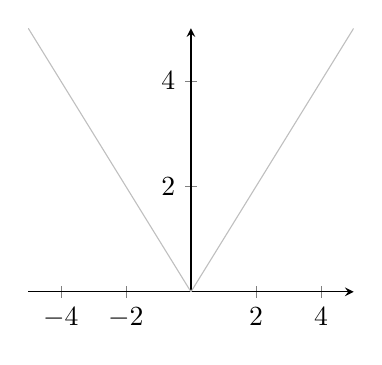
\begin{tikzpicture}
			\begin{axis}[axis lines = center]
				\addplot[color=lightgray]	{abs(x)};
			\end{axis}
		\end{tikzpicture}
	\end{center}
	\caption{The graph $y = |x|$}
\end{figure}


Once again, we present fundamental properties of absolute values, in order to provide a foundation for working with these mathematical functions.

\begin{enumerate}
	\item For any real number $x$, $|x| \ge x$ and $|x| \ge 0$.
	\item Given real numbers $x$ and $y$, $|xy| = |x| \cdot |y|$.
	\item Squaring a number strips its negative sign, and taking the positive root ensures the result will be positive. Therefore the [positive] square root of the square is the absolute value.
	\begin{align*}
		|x| = \sqrt{x^2}
	\end{align*}
\end{enumerate}

The last property is rather interesting, and can be proved. Notice for proving these simple properties of absolute values, a \emph{proof by cases} \marginnote{proof by cases} is often most effective, a proof technique in which we break all possibilities into distinct \emph{cases} or scenarios and prove the claim for each of them. Since the absolute value function behaves different for positive and negative numbers, these are naturally our cases.

\vspace{\baselineskip}
\begin{theorem}
	For any real number $x$, we have:
	
	\begin{align}
		|x| = \sqrt{x^2}
	\end{align}
\end{theorem}

\begin{proof}[Proof by Cases]
	Consider the cases when $x$ is positive, zero and negative separately. Note formally, one of these cases must be true from the trichotomy property (see the first property of inequalities above).
	
	\header{Case 1.}{$x > 0$}
	
	\begin{align*}
		\sqrt{x^2} &= x \\
		&= |x|
	\end{align*}
	
	\header{Case 2.}{$x = 0$}
	
	\begin{align*}
		\sqrt{0^2} &= 0 \\
		&= |0|
	\end{align*}
	
	\header{Case 3.}{$x < 0$}
	Assume that $x = -a$ for some positive real number $a$. Notice that $|x| = a$ Plugging this into the expression of the square root of the sqaure:
	
	\begin{align*}
		\sqrt{x^2} &= \sqrt{(-a)^2} \\
		&= \sqrt{a^2} \\
		&= |a|
	\end{align*}
\end{proof}
\vspace{\baselineskip}

At this point, we can go ahead and introduce the next major inequality. Note that we mentioned that the absolute value of the product of two numbers is the product of the absolute values, or

\begin{align*}
	|xy| = |x| \cdot |y|.
\end{align*}

Unfortunately, the same does not hold true for sums--the analogous statement is false.

\begin{align*}
	|2 + (-1)| \neq |2| + |-1|
\end{align*}

However, there is a relationship between the two quantities which can be expressed as an inequality. \\

\begin{theorem}[Triangle Inequality]
	Given real numbers $x$, $y$ the sum of the absolute values is always greater than or equal to the absolute value of the sum.
	
	\begin{align}
		|x + y| \le |x| + |y|
	\end{align}
\end{theorem}

\begin{proof}[Rough work]\let\qed\relax
	Once again, we begin with rough work to determine how to progress on the proof. In order to remove the absolute value sides, it seems reasonable to square both sides.
	
	\begin{align*}
		|x + y| &\le |x| + |y| \\
		\implies |x + y|^2 &\le (|x| + |y|)^2 \\
		\implies (x + y)^2 &\le (|x| + |y|)^2 \\
		\implies x^2 + 2xy + y^2 &\le |x|^2 + 2|x||y| + |y|^2 \\
		\implies x^2 + 2xy + y^2 &\le x^2 + 2|xy| + y^2 \\
		\implies xy &\le |xy|
	\end{align*}
	
	Notice, we arrived at a statement which is clearly true. Remember that the absolute value of any real number is always greater than or equal to the number. At this point we can write the proof.
\end{proof}
\vspace{\baselineskip}

\begin{proof}
	Consider any real number $x$ and $y$. From the basic properties of absolute values we know the product of these numbers must be less than or equal to its absolute value.
	
	\begin{align*}
		xy &\le |xy| \\
		\implies x^2 + 2xy + y^2 &\le x^2 + 2|xy| + y^2 \\
		\implies x^2 + 2xy + y^2 &\le |x|^2 + 2|x||y| + |y|^2 \\
		\implies (x + y)^2 &\le (|x| + |y|)^2 \\
		\implies |x + y|^2 &\le (|x| + |y|)^2
	\end{align*}
	
	Both terms inside the square are positive, hence we can safely square root both sides without affect the inequality.
	
	\begin{align*}
		\therefore |x + y| \le |x| + |y|
	\end{align*}
\end{proof}
\vspace{\baselineskip}

Once again in this proof, we used rough work to arrive at a statement we knew was true, and then worked backward to derive the result we wanted from this true statement. Notice we had to be more careful working backward in this example since we square rooted an inequality. Though this works when both terms inside the square are positive, it may fail spectacularly otherwise.

\begin{align*}
	&4 \ge 1 \\
	\implies (-2)^2 &\ge (1)^2 \\
	\centernot\implies -2 &\ge 1 \text{ false!}
\end{align*}

\section{Sets}
So far we have been relying on intuition to define the real numbers, the focus of our attention. Although the formal definitions of the real numbers are outside the scope of these notes, it is worth paying attention to this fundamental notion of a group of numbers. In mathematics, this concept is represented as a \emph{set}, \marginnote{set} a well-defined collection of objects. Some examples are listed below.

\begin{align*}
	S = \{\text{Saturday}, \text{Sunday}\} \\
	T = \{1, 2, 3, \dots \} \\
	R = \{n^2 : n \text{ is even} \} \\
	\phi \text{ or } \{ \}
\end{align*}

The last example presents two ways to denote the \emph{empty set}, \marginnote{empty set} the set with no elements. Notice $R$ is the set of squares of all even numbers. The `:' introduces a condition in the set definition. Since every set must be well-defined, every object is either an \emph{element} \marginnote{element} of the set or not. If set $A$ contains element $a$ but does not contain $b$, we can write

\begin{align*}
	a \in A \text{ and } b \notin A.
\end{align*}

In defining sets, we often specify the elements to be included from some \emph{universe} \marginnote{universe} of objects. However, the elements of elements not in $A$ clearly make a set as well, one which is intrinsically linked to $A$. This set is denoted the \emph{complement} \marginnote{complement} of $A$, written as $A^c$ and defined as

\begin{align*}
	A^c = \{ x \in \text{universe } : x \notin A \}
\end{align*}

Though we will explore notions of size in more depth later on, for now we define the \emph{cardinality}, \marginnote{cardinality} written as 

\begin{align*}
	|A| \text{ or } card(A),
\end{align*}

as its size. For \emph{finite} \marginnote{finite} sets, sets without an infinite number of elements, the cardinality is simply the number of elements. All such cardinalities are in the set $\mathbb{N}_0$, with 0 reserved for the empty set.

Since a set is unordered and cannot contain duplicate items, a natural definition of equality is that both sets contain the identical elements. On the other hand, if every element of set $B$ is in set $A$, then in some sense the latter set contains the former. Mathematically, we write that $B$ is a \emph{subset} \marginnote{subset} of $A$ or

\begin{align*}
	B \subseteq A.
\end{align*}

Notice under this definition, the empty set is a subset of every set. Similarly, a set is always a subset of itself. In cases where we want to exclude this possibility in explaining the relationship between the two sets, we can write $B$ is a proper subset of $A$ or 

\begin{align*}
	B \subset A
\end{align*}

which means $B \subseteq A$ but $B \neq A$. Along with the real numbers there are a handful of other important sets used to refer to classes of numbers.

\vspace{\baselineskip}
\begin{center}
	\begin{tabular}{ccc}
		\toprule
		Symbol & Name & Set \\
		\midrule
		$\mathbb{N}$ & Natural Numbers & $\{1, 2, 3, 4, \dots\}$ \\[10pt]
		$\mathbb{Z}$ & Integers & $\{\dots, -2, -1, 0, 1, 2, \dots\}$ \\[10pt]
		$\mathbb{Q}$ & Rational Numbers & $\left\{ \dfrac{p}{q} : p,q \in \mathbb{Z}\right\}$ \\[10pt]
		$\mathbb{R}$ & Real Numbers & \\
		\bottomrule
	\end{tabular}
\end{center}
\vspace{\baselineskip}

Notice we defined the natural numbers to exclude 0, but the symbol $\mathbb{N}_0$ could be used to refer to all naturals along with 0. Based on the descriptions of each of these sets, each contains the previous plus some additional elements. Therefore, we can write

\begin{align}
	\mathbb{N} \subseteq \mathbb{N}_0 \subseteq \mathbb{Z} \subseteq \mathbb{Q} \subseteq \mathbb{R}.
\end{align}

Since each set contains the previous, we may wonder what elements are in one but not the other. In some cases, this set itself might be valuable. For example all real numbers which are not rational are  referred to as as irrational, and the set which contains all such numbers the irrational numbers. This set then is a result of taking the real numbers and subtracting the rational numbers. This operation, along with a few more are formalized before for arbitrary sets $A$ and $B$.

\begin{align*}
	\emph{Subtraction. } A - B &= \{ x \in A : x \notin B \} \\
	\emph{Intesection } A \cap B &= \{ x : x \in A \text{ and } x \in B \} \\ 
	\emph{Union. } A  \cup B &= \{ x : x \in A \text{ or } x \in B \} \\
	\emph{Cartesian Product. } A  \times B &= \{ (a, b) : a \in A \text{ and } b \in B \} \
\end{align*}

The intersection is the set of all elements in both, while the union is the set of all elements in either. Two sets are called \emph{disjoint} if their intersection is the empty set meaning they have no common elements. Written out this would mean for disjoint sets $S$ and $T$,

\begin{align*}
	S \cap T = \phi
\end{align*}

The cartesian product of two sets outputs a set with a completely different structure: a set of tuples containing all possibly pairs of elements from $A$ and $B$. Unlike sets, \emph{tuples} \marginnote{tuples} are ordered list of elements. This idea of product can be extended beyond two sets.

\begin{align*}
	A \times B &= \{ (a, b) : a \in A, b \in B \} \\
	B \times A &= \{ (b, a) : a \in A, b \in B \} \\
	A \times B \times C &= \{ (a, b, c) : a \in A, b \in B, c \in C \} \\
\end{align*}

Repeated products of the same set can be abbreviated as a power, similar to the real numbers.

\begin{align*}
	A^k &= \underbrace{A \times \cdots \times A}_\text{$k$ times} \\
	&= \{ (a_1, a_2, \dots, a_k) : a_1, a_2, \dots, a_k \in A \}
\end{align*} 

One final concept that must be introduced to complete our discussion on introductory set theory is the \emph{power set} \marginnote{power set} of some set, the set which contains all possible subsets. Formally we write this as

\begin{align*}
	\emph{Power set. } \mathcal{P}(A) = \{ S : S \subseteq A \}.
\end{align*}

To ensure this section includes a proof, we end with a simple theorem about the size of a power set. We will explore another proof of this theorem later in the course.

\vspace{\baselineskip}
\begin{theorem}
	For a finite set $A$, if $|A| = n$, then its power set $\mathcal{P}(A)$ has cardinality $2^n$.
\end{theorem}

\begin{proof}[Examples]\let\qed\relax
	One way to begin working on a proof is the test the claim with examples, since they may yield insight into why the result is true.
	
	\begin{align*}
		\mathcal{\phi} &= \{ \phi \} \\
		\mathcal{P}(\{ 0, 1 \}) &= \{ \phi, \{ 0 \}, \{ 1 \}, \{ 0, 1 \}\}
	\end{align*}
	
	In each of these cases, the result holds. When the sizes of sets were 0 and 2, their power sets had sizes of 1 and 4 respectively. Notice we would also expect the number of subsets to be even, since for every subset $S \subseteq A$, $(A - S)$ is also one, and  this theorem seems to check out in that regard. At this point we can present the proof
\end{proof}
\vspace{\baselineskip}

\begin{proof}
	Since $A$ is finite and $|A| = n$ then the set must have $n$ elements. Let us arbitrarily assign labels so that
	
	\begin{align*}
		A = \{ a_1, a_2, \dots a_n \}
	\end{align*}
	
	In constructing a subset, each of these $n$ distinct elements can be chosen to either be included or excluded from the set. Since every subset can be created with these series of $n$ choices, and each choice has two options, the number of subsets is $2^n$.
\end{proof}
\vspace{\baselineskip}

A major class of proofs involves proving two sets are equal. One possible way of doing this involves showing each set is a subset of another. To prove set $S$ is a subset of $T$, we must show if $x$ is an element of $S$ then it is also an element of $T$. This would mean every element in $S$ is contained in $T$ and therefore $S \subseteq T$. To provide an example, we introduce another theorem. \\

\begin{theorem}[De Morgan's laws]
	Given two sets $A$ and $B$, the following statements are true.
	
	\begin{align}
		(A \cup B)^c &= A^c \cap B^c \\
		(A \cap B)^c &= A^c \cup B^c
	\end{align}
\end{theorem}

\begin{proof}
	Since the proof the statements are nearly identical, only the first will be proved; the second is left as an exercise. Since we are proving the equality of sets, we proceed by showing the left hand side (LHS) is a subset of the right hand side (RHS) and vice versa.
	
	\header{Part 1.}{$(A \cup B)^c \subseteq (A^c \cap B^c)$}
	
	Assume that $x \in (A \cup B)^c$, we will show $x$ is also an element of $(A^c \cap B^c)$ through a series of implications.
	
	\begin{align*}
		x \in (A \cup B)^c &\implies x \notin (A \cup B) \\
		&\implies x \notin A \text{ and } x \notin B \\
		&\implies x \in A^c \text{ and } x \in B^c \\
		&\implies x \in A^c \cap B^c
	\end{align*}
		
	\header{Part 2.}{$(A^c \cap B^c) \subseteq (A \cup B)^c$}
	
	Now assume that $x \in (A^c \cap B^c)$, we will show $x$ is also an element of $x \in (A \cup B)^c$.
	
	\begin{align*}
		x \in (A^c \cap B^c) &\implies x \in A^c \text{ and } x \in B^c \\
		&\implies x \notin A \text{ and } x \notin B \\
		&\implies x \notin (A \cup B) \\
		&\implies x \in (A \cup B)^c
	\end{align*}
	
	Since we have proved that $(A \cup B)^c \subseteq (A^c \cap B^c)$ and $(A^c \cap B^c) \subseteq (A \cup B)^c$, this is enough to show equality.
	
	\begin{align*}
		\therefore (A \cup B)^c &= A^c \cap B^c
	\end{align*}
\end{proof}
\vspace{\baselineskip}

\section{Functions}
At this point we can introduce a very special type of set which has profound uses in mathematics. This, of course, is a \emph{function}, \marginnote{function} which is a set of input-output ordered pairs which can represented as

\begin{align*}
	\{ (x, f(x)) : x \in \text{domain} \}	
\end{align*}

\begin{center}
	\begin{tabular}{rl}
		\toprule
		Term & Definition \\
		\midrule
		Domain & The set of all allowed inputs \\
		Codomain (Target Space) & The set of all allowed outputs \\
		Image (Range) & The set of all actual outputs \\
		\bottomrule
	\end{tabular}
\end{center}
\vspace{\baselineskip}

The function, then, takes an input from the domain and returns a single output in the codomain. This property of linking the domain to the codomain explains why function are often called \emph{maps}. \marginnote{map} Since the image is the set of outputs, and a subset of the codomain, it would be the set that results from applying the function to every element in the domain. Thus, for a function $f$ with domain $A$, the image is often denoted as $f(A)$.

\begin{align*}
	f(A) &= \{ f(a) : a \in A \}
\end{align*}

In defining a function, the domain and codomain must be explicitly specified, hence the following notation is often used.

\begin{align*}
	\begin{array}{llll}
		\multicolumn{4}{l}{\text{domain}} \\
		& \downarrow && \\
		f: & A & \rightarrow & B \\
		&&& \uparrow \\
		\multicolumn{4}{r}{\text{codomain}}
	\end{array}
\end{align*}

A function is called \emph{real-valued} \marginnote{real-valued} if its image is a subset of the real numbers, and thus all its outputs are real numbers. The \emph{graph} \marginnote{graph} of a function is a plot of all the input-output pairs. In working with functions there are a few elementary ways to combine them.

\begin{align}
	\emph{Addition. } (f + g)(x) = f(x) + g(x) \\
	\emph{Multiplication. } (f \cdot g)(x) = f(x) \cdot g(x) \\
	\emph{Composition. } (f \circ g)(x) = f(g(x))
\end{align}



We are often extremely interested in the image of a real-valued function. In particular, we may wonder about the nature of this set: does it have a maximum or minimum, or does the function go to infinity? Formally, a function $f: A \rightarrow \mathbb{R}$ is \emph{bounded} \marginnote{bounded} if there exists some $M \in \mathbb{R}$ such that

\begin{align*}
	|f(x)| \le M
\end{align*}

for all $x \in A$. Notice in this definition $M$ acts both a positive and negative bound since the statement is equivalent to

\begin{align*}
	-M \le f(x) \le M.
\end{align*}

It turns out that sums and products of bounded functions are bounded as well, results we prove below. Notice in these proofs we clearly state our assumptions and what we plan on showing, a technique that helps inform our approach.

\vspace{\baselineskip}
\begin{theorem}
	If functions $f$ and $g$ are bounded so are the functions $(f \cdot g)$ and $(f + g)$, formed by the sum and product of these functions respectively.
\end{theorem}

\begin{proof}
	Since $f$ and $g$ are bounded, there exist $M \in \mathbb{R}$ and $N \in \mathbb{R}$ for which 
	
	\begin{align*}
		|f(x)| \le M \text{ and } |g(x)| \le N.
	\end{align*}
	
	We hope to show there exists some bound on $|(f \cdot g)(x)|$, therefore our aim should be to express this in terms of the quantities we already have bounds for.
	
	\begin{align*}
		|(f \cdot g)(x)| &= |f(x) \cdot g(x)| \\
		&= |f(x)| \cdot |g(x)| \\
		&\le M \cdot N
	\end{align*}
	
	This shows that we have discovered a bound for the function: the product of the two bounds of our original function. Hence the function is bounded.
\end{proof}
\vspace{\baselineskip}

\begin{proof}
	Once again, assume there exist $M \in \mathbb{R}$ and $N \in \mathbb{R}$ for which
	
	\begin{align*}
		|f(x)| \le M \text{ and } |g(x)| \le N.
	\end{align*}
	
	We wish to find a bound for $|(f + g)(x)|$. However, in this case it is more tricky to decompose this into $|f(x)|$ and $|g(x)|$, and requires the triangle inequality.
	
	\begin{align*}
		|(f + g)(x)| &= |f(x) + g(x)| \\
		&\le |f(x)| + |g(x)| \\
		&\le M + N
	\end{align*}
	
	Thus, we have proved $(f + g)$, showing the sum of the bounds of the functions is the bound for the sum of the functions.
\end{proof}
\vspace{\baselineskip}

In general, approach bounding proofs by expressing the bounded functions by their definitional inequality. Then work on manipulating these inequalities through inequality or absolute value rules to obtain the desired result.

\section{Fields}
So far in our deals with $\mathbb{R}$, we have been implicitly relying on properties or axioms of arithmetic in the real numbers. Many of these properties are not exclusive to the reals, and apply to a class of algebraic structures called \emph{fields}. \marginnote{field} A field, $F$, consists of

\begin{align*}
	(F, 0, 1, +, \cdot) \text{ where } F = \{ 0, 1, \dots \} 
\end{align*}

$F$ is a set of elements in the field in including at least the additive identity 0 and the multiplicative identity 1. A field also includes two predefined binary operations, addition and multiplication, which take two inputs in $F$ and return the sum and product in $F$ respectively. These function must obey the following axioms.

\begin{align*}
	+: F \times F \rightarrow F \\
	\cdot: F \times F \rightarrow F
\end{align*}

\begin{center}
	\begin{tabular}{rp{1.5in}p{1.5in}}
		\toprule
		Name & Addition & Multiplication \\
		\midrule
		\emph{Closure} & $x + y \in F$ & $x \cdot y \in F$ \\
		\emph{Associativity} & $(x + y) + z = x + (y + z)$ & $(x \cdot y) \cdot z = x \cdot (y \cdot z)$ \\
		\emph{Commutativity} & $x + y = y + x$ & $x \cdot y = y \cdot x$ \\
		\emph{Identity} & $x + 0 = x$ & $x \cdot 1 = x$ \\
		\emph{Inverses} & each non-zero element has an additive inverse & each element has an multiplicative inverse \\[10pt]
		\emph{Distributivity} & \multicolumn{2}{c}{$x \cdot (y + z) = x 
\cdot y + x \cdot z$} \\
		\bottomrule
	\end{tabular}
\end{center}
\vspace{\baselineskip}

To clarify the inverse axioms, the first states that for any $x \in F$, there exists a $-x$, such that

\begin{align*}
	x + (-x) = 0, \, -x \in F.
\end{align*}

In this case, $-x$ is simply an element of the field, and is called the additive inverse of $x$. Commutatively, $x$ is the additive inverse of $-x$. Sometimes, the additive inverse of a field element is itself--the trivial example is 0:

\begin{align*}
	0 + 0 = 0.
\end{align*}

For non-zero elements in the field, a multiplicative inverse exists as well, which means for $x \in F - \{ 0 \}$, there exists a $x^{-1}$, such that

\begin{align*}
	x \cdot x^{-1} = 1,\, x^{-1} \in F.
\end{align*}

Similar to the additive inverse, this inverse is an element of the field and likewise can be the same number. With this axiom, we can define two new operations in the field. Subtraction amounts to adding by the additive inverse and division is multiplication by the multiplicative inverse. For field elements $x$, $y$ in some field $F$.

\begin{align}
	x - y &:= x + (-y) \\
	x / y &:= x \cdot y^{-1} \text{ given } y \neq 0
\end{align}

Notice the $:=$ here emphasizes the expression on the left is defined to be equal to the expression on the right. To avoid confusion, when working in fields, we will refrain from using subtraction and division and instead refer to the inverses.

Naturally, we may now wonder, having laid out these axioms, which sets which classes of numbers, with regularly defined addition and multiplication, constitute fields. To prove whether a set with defined operations is a field is simply a matter of checking each of the axioms. \\

\vspace{\baselineskip}
\begin{theorem}
	The natural numbers $(\mathbb{N})$ and integers $(\mathbb{Z})$ are not fields. 
\end{theorem}

\begin{proof} 
	We will prove this theorem in two parts, first dealing with the natural numbers proceeded by the integers.
	\header{Part 1. }{$\mathbb{N}$}
	The additive inverse axiom fails for all integers. Specifically, the number 1, for example, has no additive inverse since for all $n \in \mathbb{N}, 1 + n > 0$. Since 1 had no additive inverse this is not a field.
	
	\header{Part 2. }{$\mathbb{Z}$}
	The multiplicative inverse axiom fails for $2 \in \mathbb{Z}$. Once way of rigourously showing this is to notice $2 \cdot n$ is even for all $n \in \mathbb{Z}$. Therefore this value can never be 1, and hence no multiplicative inverse exists. \\
\end{proof}
\vspace{\baselineskip}

\vspace{\baselineskip}
\begin{theorem}
	The rational numbers $(\mathbb{Q})$ and real numbers $(\mathbb{R})$ with regularly defined addition and multiplication constitute fields.
\end{theorem}

\begin{proof}
	The process of proving these are fields are rather tedious, verifying each of the field axioms individually, and left as an exercise. However, note that the inverse axioms that failed for the natural numbers and integers hold for these two sets. The additive and multiplicative inverses are respectively shown below.
	
	\begin{align*}
		\frac{p}{q} \in \mathbb{Q} \rightarrow -\frac{p}{q}, \, \frac{q}{p} \in \mathbb{Q} \\
		x \in \mathbb{R} \rightarrow -x, \, \frac{1}{x} \in \mathbb{R}
	\end{align*}
\end{proof}
\vspace{\baselineskip}

These suite of axioms lead to a host of simple properties, which should feel familiar to us after working with the real numbers. We introduce an expansive theorem which lays out many of these properties.

\vspace{\baselineskip}
\begin{theorem}
	Given a field $F$ defined with addition and multiplication and three elements $x$, $y$, and $z$, the following properties must hold.
	
	\begin{align}
		x \cdot 0 = 0 \\
		\text{if } x \cdot y = 0 \text{ then } x = 0 \text { or } y = 0 \\
		-x = x \cdot (-1) \\
		(-x) \cdot (-y) = x \cdot y \\
		\text{if } x + y = x + z \text{ then } y = z \\
		\text{if } x \cdot y = x \cdot z \text{ then } y = z \text { if } x \neq 0
	\end{align}
\end{theorem}

\begin{proof}
	Proving every statement in the theorem would take up a lot of space, hence we will present proofs for the first and last statement, hopefully providing a model for approaching proofs to the remaining statements.
	
	\header{Statement 1.16. }{$x \cdot 0 = 0$}
	
	Notice that although we take this for grated in the real numbers, it is not a field axiom and must be proved. Since 0 is the additive inverse, in searching for a proof we should look to exploit its properties.

	\begin{align*}
		x \cdot 0 &= x \cdot (0 + 0) &&\emph{identity} \\
		&= x \cdot 0 + x \cdot 0 &&\emph{distributive}
	\end{align*}
	
	At this point notice by closure we know $x \cdot 0$ lies within the field. Therefore, by the inverses axiom it must have an additive inverse. Now we add this to both sides of the equation.
	
	\begin{align*}
		x \cdot 0 + x \cdot 0 &= x \cdot 0 && \\
		x \cdot 0 + x \cdot 0 + (-(x \cdot 0)) &= x \cdot 0 + (-(x \cdot 0)) && \\
		x \cdot 0 + (x \cdot 0 + (-(x \cdot 0))) &= 0  &&\emph{associative} \\
		x \cdot 0 + 0 &= 0 &&\emph{inverse} \\
		x \cdot 0 &= 0 &&\emph{identity}
	\end{align*}
	
	This is the result we were looking for. Notice instead of subtracting $x \cdot 0$ from each side, as we would in the real numbers, we added the additive inverse to  both sides. In this proof we clearly listed which axiom allowed us to make each step, and although this is not necessary, it makes it less likely to perform an operation which is not allowed.
	
	\header{Statement 1.21. }{$\text{if } x \cdot y = x \cdot z \text{ then } y = z \text { if } x \neq 0$}
	
	Once again, we attempt a direct proof based on the field axioms. Since $x \neq 0$ from the inverses axiom, we know there exists some $x^{-1} \in F$ such that
	
	\begin{align*}
		x \cdot x^{-1} = 1
	\end{align*}
	
	We simply multiply both sides of out equation with this term.
	
	\begin{align*}
		x \cdot y &= x \cdot z && \\
		x^{-1} \cdot x \cdot y &= x^{-1} \cdot x \cdot z && \\
		(x^{-1} \cdot x) \cdot y &= (x^{-1} \cdot x) \cdot z &&\emph{associativity} \\
		1 \cdot y &= 1 \cdot z &&\emph{inverse} \\
		y &= z &&\emph{identity}
	\end{align*}
	
	Once again, we have arrived at our result, hence we have proved this this statement for arbitrary fields. Notice we could approach this problem as if we were asked to prove this for real numbers. Instead of dividing both sides by $x$ we multiplied by $x^{-1}$ to arrive at the result. 
\end{proof}
\vspace{\baselineskip}

The two fields we have discussed so far have had an infinite number elements with predefined addition and multiplication operations that mirror their common usage. However, we may wonder what other fields exists, and in particular, what such a field would look like for a finite number of elements, a \emph{finite field}. \marginnote{finite field} Since a field must have at least two elements, let us attempt to construct a two element field, called the \emph{binary field}. \marginnote{binary field} Consider the field

\begin{align*}
	(S, 0, 1, +, \cdot) \text{ where } S = \{ 0, 1 \}.
\end{align*}
	
Unfortunately, we must define multiplication and addition in this field since otherwise the latter would defy the closure field axiom as

\begin{align*}
	1 + 1 &= 2 \notin S.
\end{align*}

For finite fields with a small number of elements, the most effective method of defining these operations involves writing addition and multiplication tables, providing outputs for all possible pairs of input for each function.

\vspace{\baselineskip}
\begin{center}
\begin{TAB}(e, 15pt){c|cc}{c|cc}
	+ & 0 & 1 \\
	0 & & \\
	1 & &
\end{TAB}
\hspace{15pt}
\begin{TAB}(e, 15pt){c|cc}{c|cc}
	$\cdot$ & 0 & 1\\
	0 & & \\
	1 & & \\
\end{TAB}
\end{center}
\vspace{\baselineskip}

Notice, that multiplying by 0 always returns 0 (as we proved above) and multiplying by 1 gives the same number. Similarly, adding 0 returns the same number by the identity property. 

\vspace{\baselineskip}
\begin{center}
\begin{TAB}(e, 15pt){c|cc}{c|cc}
	+ & 0 & 1 \\
	0 & 0 & 1 \\
	1 & 1 &
\end{TAB}
\hspace{15pt}
\begin{TAB}(e, 15pt){c|cc}{c|cc}
	$\cdot$ & 0 & 1\\
	0 & 0 & 0 \\
	1 & 0 & 1 \\
\end{TAB}
\end{center}
\vspace{\baselineskip}

This only leaves one output to be decided, the sum $1 + 1$. In the next theorem we prove that this is equal to 0. To do this, we introduce a new type of proof, a proof by contradiction.

\vspace{\baselineskip}
\begin{theorem}
	If $S$ is the binary field with $S = \{ 0, 1\}$, then $1 + 1 = 0$.
\end{theorem}

\begin{proof}[Proof by Contradiction]
	By the closure property of fields, we know the sum $1 + 1$ must lie within $S$ and is therefore it is either 0 or 1. Assume for sake of contradiction that it is indeed 1, so that
	
	\begin{align*}
		1 + 1 = 1.
	\end{align*}
	
	By the inverse axiom, we know that 1 has an additive inverse in the field. We now add this inverse to both sides of the equation.
	
	\begin{align*}
		1 + 1 + (-1) &= 1 + (-1) \\
		1 + 0 &= 0 \\
		1 &= 0
	\end{align*}
	
	This is clearly false since by definite a field must have distinct elements 0 and 1. Since this would be a logical consequence of letting $1 + 1 = 1$, that assumption must be false. Hence we are left only with the possibility that
	
	\begin{align*}
		1 + 1 = 0.
	\end{align*}
\end{proof}
\vspace{\baselineskip}

In a \emph{proof by contradiction}, we assume the opposite of the statement we are trying to prove, and show how this leads a result that is clearly false. This \emph{contradiction} \marginnote{contradiction} shows that our initial assumption must be false, and therefore its opposite true. In this way, we indirectly prove our claim is true by showing it cannot be false. In the last proof, we demonstrated if $1 + 1 = 1$ then $0 = 1$, which is clearly false. Therefore, we could conclude $1 + 1 \neq 1$, which meant $1 + 1 = 0$, what we wanted to show.

Moving on, we can tackle the construction of three-element field $T = \{ 0, 1, \omega \}$. Immediately, we write the addition and multiplication tables and fill out the simple rows and columns.

\vspace{\baselineskip}
\begin{center}
\begin{TAB}(e, 15pt){c|ccc}{c|ccc}
	+ & 0 & 1 & $\omega$\\
	0 & 0 & 1 & $\omega$ \\
	1 & 1 & & \\
	$\omega$ & $\omega$ &&
\end{TAB}
\hspace{15pt}
\begin{TAB}(e, 15pt){c|ccc}{c|ccc}
	$\cdot$ & 0 & 1 & $\omega$\\
	0 & 0 & 0 & 0 \\
	1 & 0 & 1 & $\omega$ \\
	$\omega$ & 0 & $\omega$ &
\end{TAB}
\end{center}
\vspace{\baselineskip}

Completing the multiplication table is simple; since every element in the field must have a multiplicative inverse, in the case of $\omega$, this must be itself. In other words, every non-zero row or column in a field multiplication table must have a single 1.

\vspace{\baselineskip}
\begin{center}
\begin{TAB}(e, 15pt){c|ccc}{c|ccc}
	+ & 0 & 1 & $\omega$\\
	0 & 0 & 1 & $\omega$ \\
	1 & 1 & & \\
	$\omega$ & $\omega$ &&
\end{TAB}
\hspace{15pt}
\begin{TAB}(e, 15pt){c|ccc}{c|ccc}
	$\cdot$ & 0 & 1 & $\omega$\\
	0 & 0 & 0 & 0 \\
	1 & 0 & 1 & $\omega$ \\
	$\omega$ & 0 & $\omega$ & 1
\end{TAB}
\end{center}
\vspace{\baselineskip}
	
This leaves the addition table to be completed, to do this we introduce a new theorem which helps complete the non-diagonal entries.

\vspace{\baselineskip}
\begin{theorem}
	For a three-element field $(T, 0, 1, +, \cdot)$ with $T = \{ 0, 1, \omega \}$ the following equation must be true.
	
	\begin{align*}
		1 + \omega &= 0 \\
	\end{align*}
\end{theorem}

\begin{proof}[Proof by Contradiction]
	Assume for sake of contradiction that $1 + \omega \neq 0$. Then, by closure the sum must either be $\omega$ or 1. We would show either case results in a contradiction.
	
	\header{Case 1.}{$1 + \omega = 1$}
	
	Since 1 is in the field, the inverses property tells us that an additive inverse exists. Adding both sides with this additive inverse we immediately see the contradiction.
	
	\begin{align*}
		1 + \omega &= 1 \\
		(-1) + 1 + \omega &= 1 + (-1) \\
		\omega &= 0
	\end{align*}
	
	Since the elements are distinct this is a contradiction.

	\header{Case 2.}{$1 + \omega = \omega$}
	
	We approach this case in a very similar way, clearing the $\omega$'s from both sides to expose a contradiction.
	
	\begin{align*}
		1 + \omega &= \omega \\
		1 + \omega + (-\omega) &= \omega + (-\omega) \\
		1 &= 0
	\end{align*}
	
	This again, is a contradiction. Therefore in the absence of any alternatives, we have proved that $1 + \omega = 0$
\end{proof}
\vspace{\baselineskip}

Note in this proof, we applied a case-by-case approach to a proof by contradiction. This is analogous to a proof by cases where we prove the result in every case, except we actually show a contradiction in each case.

\vspace{\baselineskip}
\begin{center}
\begin{TAB}(e, 15pt){c|ccc}{c|ccc}
	+ & 0 & 1 & $\omega$\\
	0 & 0 & 1 & $\omega$ \\
	1 & 1 & & 0 \\
	$\omega$ & $\omega$ & 0 &
\end{TAB}
\hspace{15pt}
\begin{TAB}(e, 15pt){c|ccc}{c|ccc}
	$\cdot$ & 0 & 1 & $\omega$\\
	0 & 0 & 0 & 0 \\
	1 & 0 & 1 & $\omega$ \\
	$\omega$ & 0 & $\omega$ & 1
\end{TAB}
\end{center}
\vspace{\baselineskip}
	
The remaining two spaces are rather easy to fill out if we remember the property that in a field

\begin{align*}
	\text{if } x + y = x + z \text{ then } y = z
\end{align*}

Fixing $x$ by focusing on an individual role or column, this tells us that different entries must be different. This is because, for example,

\begin{align*}
	\text{if } 1 + 1 = 1 + \omega \text{ then } 1 = \omega.
\end{align*}

Interestingly, this means every row and column of the addition table must contain each of the field elements. Exploiting the analogous rule for multiplication, every non-zero row or column must have every field element appear exactly once. Armed with this knowledge, we can finally complete the operator definitions, showing a three-element exists.

\begin{align*}
	T = \{ 0, 1, \omega \}
\end{align*}

\begin{center}
\begin{TAB}(e, 15pt){c|ccc}{c|ccc}
	+ & 0 & 1 & $\omega$\\
	0 & 0 & 1 & $\omega$ \\
	1 & 1 & $\omega$ & 0 \\
	$\omega$ & $\omega$ & 0 & 1
\end{TAB}
\hspace{15pt}
\begin{TAB}(e, 15pt){c|ccc}{c|ccc}
	$\cdot$ & 0 & 1 & $\omega$\\
	0 & 0 & 0 & 0 \\
	1 & 0 & 1 & $\omega$ \\
	$\omega$ & 0 & $\omega$ & 1
\end{TAB}
\end{center}
\vspace{\baselineskip}

\chapter{Language and Proofs}
\section{Statements and Connectives}
The atomic unit of mathematical reasoning is the \emph{mathematical statement} or \emph{proposition} \marginnote{proposition}, a sentence that is either true or false. This requirement is based on the \emph{principle of bivalence.} For a statement, its \emph{truth value} is whether it is true or false. Examples of statements are given below.

\begin{align*}
	P &\equiv \text{$\pi$ is rational} \\
	Q &\equiv \text{$x^2 + x + 1$ has a real solution} \\
	R &\equiv \text{July 4, 1776 was a Thursday} \\
\end{align*}
 
In our examples, the first statement is false while the other two are true. On the other hand ``let them eat cake'' is not a mathematical statement. These statements can be combined with logical connectives to express more complicated thoughts, which are listed below.

\vspace{\baselineskip}
\begin{center}
	\begin{tabular}{ccc}
		\toprule
		Name & Usage & Meaning \\
		\midrule
		Negation & $\neg P$ & not $P$ \\
		Conjunction & $P \wedge Q$ & $P$ and $Q$ \\
		Disjunction & $P \lor Q$ & $P$ or $Q$ \\
		Conditional & $P \implies Q$ & if $P$ then $Q$ \\
		Biconditional & $P \iff Q$ & $P$ if and only if $Q$ \\
		\bottomrule
	\end{tabular}
\end{center} 
\vspace{\baselineskip}

Similar to defining operators in a finite field, we provide rigorous definitions for these logical connectives by showing whether the compound statement is true of false for every possible set input. Fortunately there are very few possible inputs since each statement can either be true or false. In composing a table, called a \emph{truth table}, \marginnote{truth table} we let each row correspond to a unique input.

\vspace{\baselineskip}
\begin{center}
	\begin{TAB}(c, 50pt){cc}{c|cc}
		$P$ & $\neg P$ \\
		T & F \\
		F & T \\
	\end{TAB}
\end{center}
\vspace{\baselineskip}

Notice this truth table shows completely negation, since it tells us how the statement behaves given every input. In this case, if a statement is true its negation is false and if a statement is false its negation is true. In English, then, the negation of a statement would be its opposite. The truth tables for the remaining connective are given below; notice each require two inputs and thus have four possible inputs.

\vspace{\baselineskip}
\begin{multicols}{2}
	\begin{center}
	\begin{TAB}(c, 50pt){ccc}{c|cccc}
		$P$ & $Q$ & $P \wedge Q$ \\
		T & T & T \\
		T & F & F \\
		F & T & F \\
		F & F & F \\
	\end{TAB}
	\end{center}
	
	\begin{center}
	\begin{TAB}(c, 50pt){ccc}{c|cccc}
		$P$ & $Q$ & $P \implies Q$ \\
		T & T & T \\
		T & F & F \\
		F & T & T \\
		F & F & T \\
	\end{TAB}
	\end{center}
	
	\begin{center}
	\begin{TAB}(c, 50pt){ccc}{c|cccc}
		$P$ & $Q$ & $P \lor Q$ \\
		T & T & T \\
		T & F & T \\
		F & T & T \\
		F & F & F \\
	\end{TAB}
	\end{center}

	\begin{center}
	\begin{TAB}(c, 50pt){ccc}{c|cccc}
		$P$ & $Q$ & $P \iff Q$ \\
		T & T & T \\
		T & F & F \\
		F & T & F \\
		F & F & T \\
	\end{TAB}
	\end{center}
\end{multicols}
\vspace{\baselineskip}

These truth tables provide complete definitions for each of these operators, but fail to provide very much intuition.

\begin{itemize}
	\item \emph{Negation:} As mentioned before, if $R$ is true its negation is false and vice versa. The simple interpretation of this that $\neg R$ is the opposite of $R$.
	\begin{align*}
		P &\equiv \text{$\pi$ is rational} \\
		\neg P &\equiv \text{$\pi$ is not rational} \\
		Q &\equiv \sqrt{2} > 0 \\
		\neg Q &\equiv \sqrt{2} \le 0
	\end{align*}
	
	\item \emph{Conjunction:} $P \wedge Q$ is true only when both $P$ and $Q$ are true, which matches with we think about ``and.''
	\begin{align*}
		P &\equiv \text{$\sqrt{2}$ is irrational} \\
		Q &\equiv \text{$(x^2 = 2)$ holds when $x = \sqrt{2}$} \\
		P \wedge Q &\equiv \text{$\sqrt{2}$ is irrational and a solution to $x^2 = 2$}
	\end{align*}

	\item \emph{Disjunction:} $P \lor Q$ is true when either $P$, $Q$, or both $P$ and $Q$. Another way to think about this is that  $P \lor Q$ is only false when both statements $P$ and $Q$ are both false. There is a slight difference between this logical ``or'' and the one in everyday usage; often times ``or'' in English can mean one or the other but not both, which is called the \emph{exclusive-or} in mathematics.
	\begin{align*}
		P &\equiv \text{$x$ is positive} \\
		Q &\equiv \text{$x$ is negative} \\
		P \lor Q &\equiv \text{$x$ is positive or negative} \\
		&\equiv \text{$x$ is nonzero}
	\end{align*}
	
	\item \emph{Conditional:} This connective is essential in proofs, and thus is worth taking closer look at.
	\begin{align*}
	\begin{array}{lll}
		\multicolumn{3}{l}{\text{hypothesis}} \\
		\downarrow && \\
		P & \implies & Q \\
		&& \uparrow \\
		\multicolumn{3}{r}{\text{conclusion}}
	\end{array}
	\end{align*}
	The first statement is called the \emph{hypothesis}\marginnote{hypothesis} and the second statement the \emph{conclusion}\marginnote{conclusion}. The statement $(P \implies Q)$, interpreted as either
	
	\vspace{\baselineskip}
	\begin{center}
			``if $P$ then $Q$'' or \\
			``$P$ implies $Q$,''
	\end{center}
	\vspace{\baselineskip}
	
	  means when $P$ (the hypothesis) is true, $Q$ (the conclusion) must be true as well. On the other hand, when $P$ is false, it does matter whether $Q$ is true or false, and the statement is true in either case. Once again, the only time a conditional is false is when $P$ is true but $Q$ is false.
	  
	  \item \emph{Biconditional:} A biconditional $(P \iff Q)$ is true when both $P$ and $Q$ have the truth value and false they do not. Therefore, if the biconditional is true the statements $P$ and $Q$ are logically interchangeable since both are true or false together. For this reason, $P$ and $Q$ can be said to be ``logically equivalent.'' This concept is expressed as
	  	  
	  \begin{align*}
	  	P \iff Q \text{ and } P \equiv Q,
	  \end{align*}
	  
	  where the second notation is traditionally used to indicate the two logical compound expressions are equivalent, especially when one side might itself contain the biconditional connective.
\end{itemize}

It turns out that from these logical connective we can construct many expressions which are identical. We prove a few of the important logical equivalences. \\

\begin{theorem}[De Morgan's laws]
	For two logical statements $R$ and $S$, the following equivalences are true.
	
	\begin{align}
		\neg(R \wedge S) &\equiv \neg R \lor \neg S \\
		\neg(R \lor S) &\equiv \neg R \wedge \neg S
	\end{align}
\end{theorem}

\begin{proof}
	The general way to prove logical statements are equivalent is to construct truth tables and show both statements have identical outputs for the same inputs. In order to avoid receptiveness, we will do this for the first statement and leave the proof for the second as an exercise.
	
	\vspace{\baselineskip}
	\begin{center}
		\begin{tabular}{cccc}
			$R$ & $S$ & $R \wedge S$ & $\neg(R \wedge S)$ \\
			\midrule
			T & T & T & F \\
			T & F & F & T \\
			F & T & F & T \\
			F & F & F & T \\
		\end{tabular}
	\end{center}
	\vspace{\baselineskip}
	
	This gives us the truth table for the left hand side of the equation. We follow the same process, slow building up the right hand side.
	
	\vspace{\baselineskip}
	\begin{center}
		\begin{tabular}{ccccc}
			$R$ & $S$ & $\neg R$ & $\neg S$ & $\neg R \lor \neg S$ \\
			\midrule
			T & T & F & F & F \\
			T & F & F & T & T \\
			F & T & T & F & T \\
			F & F & T & T & T \\
		\end{tabular}
	\end{center}
	
	Since $(\neg R \lor \neg S)$ and $\neg(R \wedge S)$ are true and false together, given the same inputs (have identical columns) the two statements are logically equivalent. \\
\end{proof}
\vspace{\baselineskip}

\vspace{\baselineskip}
\begin{theorem}
	The following logical equivalences are true.
	
	\begin{align}
		P \iff Q &\equiv (P \implies Q) \wedge (Q \implies P) \\
		P \implies Q &\equiv (\neg Q \implies \neg P) \\
		P \implies Q &\equiv \neg (P \wedge \neg Q)
	\end{align}
\end{theorem}

\section{Predicates and Quantifiers}

Even after the application of connectives, statements are rather limited and specific, and so to express classes of statements, \emph{predicates} \marginnote{predicates} are used. A predicate with variables is an expression which is either true or false when its variables are supplied. Since predicates are not statements until its variables are defined, they are sometime called \emph{open statements}.

\begin{align*}
	P(n) = n \text{ is even}
\end{align*}

Above is an example of such a predicate; although it currently is neither true nor false, as soon as $P$ is given a reasonable input its truth value is defined.

\begin{align*}
	P(0) \text{ is true} \\
	P(1) \text{ is false} \\
	P(2) \text{ is true} \\
	\dots
\end{align*}

Notice the truth value changes as a function of the input, though we need only consider inputs for which it is well-defined. For example, in this case, the expression $P(\pi)$ makes no sense since even and odd are not defined for real numbers.

Having introduced this machinery, we can return to DeMorgan's laws and explain its connection to the identically named rules for sets. For two sets $A$ and $B$, consider the following statements.

\begin{align*}
	R(x) &= x \in A \\
	S(x) &= x \in B
\end{align*}

From DeMorgan's laws, we know the following logical equivalence is true.

\begin{align*}
	\neg[R(x) \wedge S(x)] &\equiv \neg R(x) \lor \neg S(x) \\
\end{align*}

We will translate both sides into the language of set theory.
 
\begin{align*}
	\neg[R(x) \wedge S(x)] &\equiv \neg[(x \in A) \wedge (x \in B)] \\
	&\equiv \neg[x \in (A \cap B)] \\
	&\equiv x \notin (A \cap B) \\
	&\equiv x \in (A \cap B)^c
\end{align*}

\begin{align*}
	\neg R(x) \lor \neg S(x) &\equiv \neg(x \in A) \lor \neg(x \in B) \\
	&\equiv x \notin A \lor x \notin B \\
	&\equiv x \in A^c \lor x \in B^c \\
	&\equiv x \in A^c \cup B^c
\end{align*}

\begin{align*}
	\therefore (A \cap B)^c = A^c \cup B^c
\end{align*}

Similarly, with these defined statements,

\begin{align*}
	\neg[R(x) \lor S(x)] &\equiv \neg R(x) \wedge \neg S(x) \\
	\text{means } (A \cup B)^c &= A^c \cap B^c
\end{align*}

So far we have only discussed whether statements are true for individual inputs, but often times we are interested in the behavior of a predicate over a set of inputs. To do this, we introduce two quantifiers.

\begin{align*}
	\emph{Universal. } \forall x \in S &\equiv \text{ ``for all $x$ in $S$''} \\
	\emph{Existential. } \exists x \in S &\equiv \text{ ``there exists an $x$ in $S$''}
\end{align*}

Attaching either a universal quantifier or existential quantifier to a predicate makes it a statement.

\begin{align*}
	(\forall x \in S)P(x) \equiv &\text{ ``for all $x$ in $S$ such that} \\
	& \text{\quad $P(x)$ is true''} \\
	(\exists x \in S)P(x) \equiv &\text{ ``there exists an $x$ in $S$ such that} \\
	& \text{\quad $P(x)$ is true''}
\end{align*}

In English these quantifiers can often be disguised, but are commonly used when talking about mathematical statements. A predicate with multiple variables can have multiple quantifiers, where order matters.

\begin{align*}
	S &= (\forall x \in \mathbb{R})(\exists M \in \mathbb{R})(|x^2| \le M) \\
	&= \text{for all real numbers $x$, there exists a real $M$ such that $|x^2| \le M$} \\
	T &= (\exists M \in \mathbb{R})(\forall x \in \mathbb{R})(|x^2| \le M) \\
	&= \text{there exists a real $M$ such that for all real $x$, $|x^2| \le M$}
\end{align*}

The first statement means that for any real input of $x^2$, we can find a $y$-value which is more extreme that it. This is trivially true since any finite input of the function is finite, take for example

\begin{align*}
	M = x^2 + 1.
\end{align*}

On the other hand, the second statements says there is some bound $M$ for which all values in the image of $f(x) = x^2$ lie between $-M$ and $M$. Note this is identical to the definition of a bounded function we discussed earlier, only written in the form of a statement. Now consider the negation of this statement. To argue a function is not bounded is to should for all bounds $M$ we can chose at least one point which exceeds this bound.

\begin{align*}
	\neg T &= (\forall M \in \mathbb{R})(\exists x \in \mathbb{R})(x^2 > M)
\end{align*}

If we compare the definition of bounded with its negation we notice an interesting relationship, where, in addition to the predicate being negated, all universal quantifiers turn into existential ones and vice versa. This is formalized below.

\vspace{\baselineskip}
\begin{theorem}
	When negating a quantified predicate, flip the quantifiers in addition to negating the predicate.
	
	\begin{align}
		\neg [(\forall x \in S)P(x)] &\equiv (\exists x \in S)\neg P(x) \\
		\neg [(\exists x \in S)P(x)] &\equiv (\forall x \in S)\neg P(x) 
	\end{align}
\end{theorem}

\section{Proving Existential Statements}

The simplest class of statements we need to prove are those with existential quantifiers; those of the form

\begin{align*}
	(\exists x \in S)P(x).
\end{align*}

To prove such a statement is rather straightforward and usually involves finding the $x$ for which the claim is true. For example, we can prove the following statement, which is sufficient to show the irrational numbers do not obey closure under regular addition and therefore cannot be considered a field.

\vspace{\baselineskip}
\begin{theorem}
	There exist two irrational numbers $r$ and $s$ for which $r$ + $s$ is rational.
\end{theorem}
\begin{proof}
	Expressed as a logical statement, we are interested in the statement
	
	\begin{align*}
		(\exists r, s \in \mathbb{R} - \mathbb{Q})(r - s \in \mathbb{Q}).
	\end{align*}
	
	We will prove this existentially qualified statement by fining such a pair of irrational $r$ and $s$ for which their sum is irrational. Consider now:
	
	\begin{align*}
		\begin{cases}
			r = \pi \\
			s = -\pi \\
		\end{cases}
	\end{align*}
	
	\begin{align*}
		r - s = \pi + (-\pi) = 0
	\end{align*}
	
	Since we have found at least one pair of elements for which this statement is true, we have proved that the sum of two irrational numbers can be rational.
\end{proof}
\vspace{\baselineskip}

Of course, explicitly finding an example which satisfies the statement may not be as easy. Sometimes it is possible to show such an example must exist without actually finding it in a type of proof called a \emph{non-constructive proof}. \marginnote{non-constructive} The most famous example of such a proof is given below.

\vspace{\baselineskip}
\begin{theorem}
	There exist two irrational numbers $r$ and $s$ for which $r^s$ is rational.
\end{theorem}

\begin{proof}[Proof by Cases]
	This proof seems nearly impossible to attempt directly. The irrational numbers are a very diverse set and finding a starting point is elusive. Instead, we attempt a non-constructive proof with a trick.
	
	\header{Case 1. }{$\sqrt{2}^{\sqrt{2}}$ is irrational}
	Notice what happens when this number is raised to the power of $\sqrt{2}$.
	
	\begin{align*}
		\left( \sqrt{2}^{\sqrt{2}} \right)^{\sqrt{2}} &= \sqrt{2}^{\sqrt{2} \cdot \sqrt{2}} \\
		&= \sqrt{2}^2 \\
		&= 2 \in \mathbb{Q}
	\end{align*}
	
	Therefore if $\sqrt{2}^{\sqrt{2}}$ is irrational, then we have found two irrational numbers for which their power is rational.
	
	\header{Case 2. }{$\sqrt{2}^{\sqrt{2}}$ is rational}
	
	It turns out that if this case is correct, then our proof is automatically done, since the square root of two, an irrational number, when raised to the power of itself is rational.
	
	Ultimately, we have shown that either
	
	\begin{align*}
		\left( \sqrt{2}^{\sqrt{2}} \right)^{\sqrt{2}} \text{ or } \sqrt{2}^{\sqrt{2}}
	\end{align*}
	
	must be rational. Although we do not know which case is correct, one of them must be true and thus there must exist two irrational numbers who power is rational. (In case you were still curious, it turns out the first case is correct.)
\end{proof}
\vspace{\baselineskip}

We will now introduce \emph{even} and \emph{odd} integers \marginnote{even, odd} and use this an an opportunity to prove statements about this property.

\begin{align*}
	\emph{Even. } x \text{ is even means } x = 2k \text{ for some } k \in \mathbb{Z} \\
	\emph{Odd. }x \text{ is odd means } x = 2k + 1 \text{ for some } k \in \mathbb{Z}
\end{align*}

Notice with definition every integer is either even or odd but not both. The sets of even and odd numbers look as follows

\begin{align*}
	\mathbb{Z}_e &= \{ \dots, -4, -2, 0, 2, 4, \dots \} \\
	\mathbb{Z}_o &= \{ \dots, -3, -1, 1, 3, 5, \dots \}
\end{align*}

where $\mathbb{Z}_e$ denotes the even integers and $\mathbb{Z}_o$ the odd integers. We will leave our discussion of \emph{parity}, \marginnote{parity}, the property of being either even or odd, here for now.

\section{Unary Proofs}

Despite this discussion about proving existential quantifiers, we are primarily interested in proving or disproving statements with universal quantifiers. That is, we prefer more general results about all natural numbers, all integers, or all real numbers. To disprove a statement, we can prove its negation. For a universally quantified statement, these have the following forms.

\begin{align*}
	P &\equiv (\forall x \in S)P(x) \\
	\neg P &\equiv (\exists x \in S)\neg P(x).
\end{align*}

Hence, proving such a statement false amounts to finding at least one example for which the result fails to hold. As we showed above, this can either be done explicitly or implicitly (non-constructively). In the scenario where we find such case, we call it a \emph{counterexample}. \marginnote{counterexample} Since the negation of a universal quantifier is existential, only one counterexample is needed to prove the entire claim false.


It follows that we may now want to explore techniques to help prove these statements true. Of course, we usually deal with infinite sets and it is impossible to manually verify the predicate holds for all possible inputs. However, once we realize the majority of results fall within one of three classes of statements, 

\begin{align*}
	S_1 &\equiv (\forall x \in S)P(x), \\
	S_2 &\equiv (\forall x \in S)[P(x) \implies Q(x)], \text{ and} \\
	S_3 &\equiv (\forall x \in S)[P(x) \iff Q(x)],
\end{align*} 

we can apply the tools mathematical logic to discover more efficient methods to approach these proofs. But first, we provide examples of statements  of this form statements we have already encountered.

\vspace{\baselineskip}
\begin{center}
	\begin{tabular}{rp{0.6\linewidth}}
		\toprule
		Type & Examples \\
		\midrule
		$P(x)$ & for all real numbers $x$, $\sqrt{x^2} = |x|$ \\
		& for all $x, y \in \mathbb{R}$, $|x| + |y| \ge |x +y|$ \\
		& for any finite set $S$, the size of $\mathcal{P}(S)$ is $2^{|S|}$ \\
		& for any statements $S$ and $T$, $\neg(S \wedge T) \equiv \neg S \wedge \neg T $ \vspace{0.25\baselineskip} \\
		$P(x) \implies Q(x)$ & if $x = y$ and $x, y > 0$ then their arithmetic mean equals their geometric mean. \\
		& if $b^2 - 4ac \ge 0$ then a quadrative equation has at least one solution \\
		& if $F$ is a field with $x, y \in F$, then $(x + y) \in F$ \\
		\bottomrule
	\end{tabular}
\end{center}
\vspace{\baselineskip}

We first begin our examination of proof techniques with statements of the form

\begin{align*}
	(\forall x \in S)P(x).
\end{align*}

Notice that these statements are actually of the form

\begin{align*}
	(\forall x \in S)[H(x) \implies P(x)],
\end{align*}

where $H(x)$ represents many of the definitions and assumptions we take for granted. For example, in proving the triangle inequality, we assumed that the absolute value function was defined in a particular way, along with a few axioms of the real numbers. However since the hypotheses are not meaningful in the sense that they provides any significant information apart from the generally accepted rules, they are acceptable to omit. The two main methods of proving such a statement are a direct proof and a proof by contradiction. In the former,we derive the statement directly from those which are true. An example of such a proof is given below.

\vspace{\baselineskip}
\begin{theorem}
	For any real number $x$ the following inequality is always true.
	
	\begin{align}
		|x| + \frac{1}{|x|} \ge 2
	\end{align}
\end{theorem}

\begin{proof}
	It turns out that this statement is rather useful, and rather appears frequently in other places. This statement is rather easy to prove as well, since it appears to be a special case of the arithmetic-geometric inequality. Take:
	
	\begin{align*}
		\begin{cases}
			a = |x| \\
			b = 1 / |x|
		\end{cases}
	\end{align*}
		
	Since both $a$ and $b$ are greater than 0 we can apply the special case of the theorem which hold for positive numbers.
	
	\begin{align*}
		a + b &\ge 2 \sqrt{ab} \\
		&= 2 \sqrt{|x| \cdot 1 / |x|} \\
		&= 2 \\
		\therefore |x| + \frac{1}{|x|} &\ge 2
	\end{align*}
\end{proof}
\vspace{\baselineskip}

While a direct proof is rather straightforward, it can difficult to see how to proceed when confronted with a statement. In this case, a \emph{proof by contradiction} can be used: assume the negation of the statement and show that it must be wrong. Remember that a either a statement or its negation must be true, therefore showing the negation to be false is equivalent to proving the statement true. An example where a direct proof might be difficult is given below.

\vspace{\baselineskip}
\begin{theorem}
	For any list of real numbers, there must be at least one value which is a large as the average. Alternatively, this can be expressed as:
	
	\begin{align}
		\max(x_1, x_2, \dots, x_n) \ge \frac{x_1 + x_2 + \dots + x_n}{n}
	\end{align}
\end{theorem}

\begin{proof}[Proof by Contradiction]
	Attempting a direct proof seems unwise; instead, we approach this with a proof by contradiction. Assume there exist a list of real numbers for which every number is less than the average. Therefore we would have
	
	\begin{align*}
		x_1, x_2, \dots, x_n < \frac{x_1 + x_2 + \dots + x_n}{n}
	\end{align*} 
	
	Since we have a bound on every single term, we can find a bound on the sum.
	
	\begin{align*}
		x_1 + x_2 + \dots + x_n &< \underbrace{\left( \frac{x_1 + \dots + x_n}{n} \right)}_\text{for each of $n$ terms} + \dots \\
		&= n \left( \frac{x_1 + \dots + x_n}{n} \right) \\
		&= x_1 + x_2 + \dots + x_n
	\end{align*}
	
	At this point, we have arrive at the conclusion that the sum of the numbers is less than itself. This is a contradiction, and thus such a list cannot exist.
\end{proof}

Notice in this case, the result we where trying to prove was actually doubly quantified. Formally, we would write

\begin{align*}
	(\forall \, (x_1, \dots, x_n) \in \mathbb{R}^n)(\exists \, x_i \in (x_1, \dots, x_n))[x_i \ge \mean(x_1, \dots, x_n)] \equiv \\
	\text{for all lists of real numbers, there exists some element in the list for which...}
\end{align*}

In proving this statement via contradiction, we need to be careful in taking the negation, remembering to swap quantifier types. Our negation is then

\begin{align*}
	(\exists \, (x_1, \dots, x_n) \in \mathbb{R}^n)(\forall \, x_i \in (x_1, \dots, x_n))[x_i \ge \mean(x_1, \dots, x_n)] \equiv \\
	\text{there exists some list of real numbers for which all elements are...}
\end{align*}

Notice this is precisely what we assumed during the proof, thus making it logically sound. Proofs by contradiction are also rather useful for claims of irrationality. Although rational numbers are well-defined and easy to work with, while the irrationals are less so. And example of such a proof is below.

\vspace{\baselineskip}
\begin{theorem}
	The square root of two $(\sqrt{2})$ is irrational.
\end{theorem}

\begin{proof}[Proof by Contradiction]
	Above we used the fact that the square root of 2 was irrational, but we never proved it. We do so now using a proof by contradiction. Assume, then, that the square root of two is rational so we can write
	
	\begin{align*}
		\sqrt{2} = \frac{p}{q}
	\end{align*}
	
	for $p$ and $q$ in lowest terms. We emphasize this point here, that the fraction is in lowest terms, since ever rational number can be written in this way. At this point we square both sides to remove the square root.
	
	\begin{align*}
		2 = \frac{p^2}{q^2} \\
		\implies 2 q^2 = p^2
	\end{align*}
	
	Notice that $p^2$ can be expressed as two times an integer so it must even. It follows that $p$ must also be even, since if it was odd so would its square. therefore, for some $k \in \mathbb{Z}$, we can write
	
	\begin{align*}
		p = 2k \\
		2 q^2 = (2k)^2 \\
		\implies q^2 = 2k^2
	\end{align*}
\end{proof}

This means that $q^2$ is also even and so $q$ must be as well. This however is a contradiction, since we assumed the fraction was in reduced form and therefore both the number and denominator cannot be divisible by two.
\vspace{\baselineskip}


\section{Conditional Proofs}

In the last chapter, we also mentioned two other classes of statements we are likely to prove.

\begin{align*}
	S_2 &\equiv (\forall x \in S)[P(x) \implies Q(x)] \\
	S_3 &\equiv (\forall x \in S)[P(x) \iff Q(x)]
\end{align*}

Despite being slightly more complex, many of the techniques we see in this section are similar to those we explored earlier. We now tackle the second class of statements of the form $P(x) \implies Q(x)$. A summary of the three techniques we will use throughout the course of the section are below.

\begin{center}
	\begin{tabular}{ccc}
		\toprule
		Method & Approach & Statement \\
		\midrule
		Direct & assume $P(x)$, show $Q(x)$ & $P(x) \implies Q(x)$ \\
		Contrapostive & assume $\neg Q(x)$, show $\neg P(x)$ & $\neg Q(x) \implies \neg P(x)$ \\
		Contradiction & assume $P(x) \wedge \neg Q(x)$, show contradiction & $\neg[P(x) \wedge \neg Q(x)]$ \\
		\bottomrule
	\end{tabular}
\end{center}
\vspace{\baselineskip}

Once again, the most straightforward approach is to attempt a direct proof. For an example, we can prove the following theorem rather simply, assuming the hypothesis and manipulating it to arrive at the conclusion.

\vspace{\baselineskip}
\begin{theorem}
	The sum and product of two even numbers are both even. 
\end{theorem}

\begin{proof}
	We proceed with a direct proof; to help see the hypothesis and conclusion we can write this out as a logical statement.
	
	\begin{align*}
		(\forall n, m \in \mathbb{Z})[(n, m \in \mathbb{Z}_e) \implies (n + m, nm \in \mathbb{Z}_e)]
	\end{align*}
	
	We're using shorthand here where $n, m \in \mathbb{Z}$ is a more compact way of writing $n \in \mathbb{Z}$ and $m \in \mathbb{Z}$. Nonetheless, our assumptions and desired conclusion are now clear, and we can proceed. Assume $n, m$ are even so that for some $k_1, k_2 \in \mathbb{Z}$:
	
	\begin{align*}
		\begin{cases}
			n = 2 k_1 \\
			m = 2 k_2
		\end{cases}
	\end{align*} 
	
	We will now express both the product and sum in terms of $k_1$ and $k_2$.
	
	\begin{align*}
		n + m &= 2 k_1 + 2 k_2 \\
		&= 2 (k_1 + k_2) \\
		nm &= (2 k_1)(2 k_2) \\
		&= 4 k_1 k_2 \\
		&= 2 (2 k_1 k_2)
	\end{align*}
	
	Since the sum and product can be expressed as 2 times some integer we can conclude they are both even. For sake of completeness, we introduce a more general theorem. The proof of each of its remaining parts are very similar and left as an exercise.
\end{proof}
\vspace{\baselineskip}

\begin{theorem}
	For integers $n, m \in \mathbb{Z}$ the following conditions determine whether the sum or product is even or odd.
	
	\begin{itemize}
		\item if $n$ is even and $m$ is even, $n + m$ is even and $nm$ is even
		\item if $n$ is even and $m$ is odd, $n + m$ is odd and $nm$ is even
		\item if $n$ is odd and $m$ is even, $n + m$ is odd and $nm$ is even
		\item if $n$ is odd and $m$ is odd, $n + m$ is even and $nm$ is odd
	\end{itemize}
\end{theorem}
\vspace{\baselineskip}

This theorem can be summarized with the following two tables,

\vspace{\baselineskip}
\begin{center}
\begin{TAB}(e, 15pt){c|cc}{c|cc}
	+ & e & o \\
	e & e & o \\
	o & o & e
\end{TAB}
\hspace{15pt}
\begin{TAB}(e, 15pt){c|cc}{c|cc}
	$\cdot$ & e & o\\
	e & e & e \\
	o & e & o \\
\end{TAB}
\end{center}
\vspace{\baselineskip}

which are oddly reminiscent of the addition and multiplication tables in a binary field. In fact, if we constructed a field 

\begin{align*}
	(F, e, o, +, \cdot) \text{ with } F = \{ e, o \},
\end{align*}

its operations would be defined in exactly this way, with $e$ as the additive identity and $o$ the multiplicative identity. For now, we leave this connection as an unlikely coincidence, but we will revisit this after tackling modular arithmetic.

\begin{align*}
	P(x) \implies Q(x) \equiv \underbrace{\neg Q(x) \implies \neg P(x)}_\text{contrapositive}
\end{align*}

Above is one of the logical equivalences we proved earlier, the right hand side is called is called the \emph{contrapositive} or \emph{contraposition}. \marginnote{contrapositive, contraposition} This fundamental equivalence tells us that to prove a conditional we can instead prove the contrapositive by assuming the negation of the conclusion and deriving the negation of the hypothesis. The canonical example is the set of statements:

\vspace{\baselineskip}
\begin{center}
	\emph{Original.} if it rains the streets are wet \\
	\emph{Contrapositive.} if the streets are dry then it did not rain
\end{center}
\vspace{\baselineskip}


This is useful when the negations of the hypothesis and conclusions are better defined or easier to work with. This often occurs when we have statements with ``not equal to'' and in claims about parity.

\vspace{\baselineskip}
\begin{theorem}
	If the $n^2$ is even, then $n$ must be even as well. Similarly, if $n^2$ is odd, then $n$ must be odd. In other words, $n^2$ always has the same parity as $n$/
\end{theorem}

\begin{proof}[Proof by Contrapositive]
	We will show the two parts of this theorem separately, and prove the first with the contrapositive. The second part is left as an exercise.
	
	\header{Part 1.}{$n^2$ is even}
	We can write out our statement formally, so we can see its hypothesis and conclusion more easily. This also makes it easy to see the contrapositive.
	
	\begin{align*} 
		(\forall n \in \mathbb{Z})(n^2 \text{ is even } \implies n \text{ is even}) \\
		(\forall n \in \mathbb{Z})(n \text{ is odd } \implies n^2 \text{ is odd})
	\end{align*}
	
	The contrapositive is substantially easier to prove; assume that $n$ is odd so that for some integer $k$, $n = 2k + 1$. We can then express the square in terms of $k$.
	
	\begin{align*}
		n^2 &= (2k + 1)^2 \\
		&= 4k^2 + 4k + 1 \\
		&= 2(2k^2 + 2) + 1
	\end{align*}
	
	Since $n^2$ can also be expressed as two times an even number it must also be odd. Therefore, we have proved our original statement. Notice we used this fact in the proof that the square root of two was irrational, though only casually proved it.
\end{proof}

\vspace{\baselineskip}

\begin{theorem}
	For any two positive numbers $x$ and $y$,
	
	\begin{align*}
		\text{if } x \neq y \text{ then } x^2 \neq y^2
	\end{align*}
\end{theorem}

\begin{proof}
	This result means that different positive numbers must have different squares. This fact was actually essential in many of our proofs, since it means that given we are working with positive numbers, we are allowed to square root both sides of the equation without affecting the equality. In other words, knowing each positive number has a unique squares allows us to work backward and determine a number uniquely from its square. It turns out this property is not unique to the squaring function but rather applies to an entire class of function; but for now we stick with proving this statement, or rather its contrapositive.
	
	\begin{align*}
		(\forall x, y \in \mathbb{R})(x^2 = y^2 \implies x = y)
	\end{align*}
	
	The proof at this point is rather straightforward, and involves simplifying the hypothesis to reach the conclusion.
	
	\begin{align*}
		x^2 &= y^2 \\
		\implies \sqrt{x^2} &= \sqrt{y^2} \\
		\implies |x| &= |y| \\
		\implies x &= y
	\end{align*}
\end{proof}
\vspace{\baselineskip}

The final proof technique, as outlined earlier, is a proof by contradiction. Remember the only case in which a conditional is false is when the hypothesis is true and the conclusion is false. Therefore its negation is as follows.

\begin{align*}
	\neg[P(x) \implies Q(x)] \equiv P(x) \wedge \neg Q(x)
\end{align*}

Once again, in a proof by contradiction the idea is to assume the negation and show a contradiction. Since we are interested in proving a conditional, we assume the hypothesis and the negation of the conclusion, showing this yields a contradiction.

%\chapter{Mathematical Induction}
%\chapter{Bijections and Cardinality}
%\chapter{Divisibility}
%\chapter{Modular Arithmetic}




\end{document}